% 来源: 19c9fbc5-1cc2-87c7-8000-00008e09ec59_3.1_网络拓扑.pdf
% 提取时间: 2026-02-28T22:51:50+08:00

3.1 网络拓扑
相对于点到点连接，网络需要把更多的节点连接起来，为此我们先学习连接的艺术 - Topology
网络拓扑（Network Topology）是指网络中节点（如计算机、服务器、交换机、路由器等）和通信链路
（如电缆、无线连接等）的物理或逻辑排列方式。它决定了数据如何在网络中传输，并直接影响网络的
性能、可靠性和可扩展性。
网络拓扑结构定义了计算节点之间的物理连接方式。良好的拓扑设计需要平衡三个核心指标：链路成本
（布线复杂度）、网络直径（最远通信距离）和对分带宽（网络分割时的最小连接带宽）。我们系统分
析主流拓扑结构的数学特性与工程实现。
拓扑可分为两类：直接网络和间接网络。
直接网络中，处理节点直接连接到交换结构，即交换结构分布在处理节点之间。直接网络包括 环面和超
立方体，以及扁平化蝴蝶等高基数拓扑；
间接网络中，端点网络独立于端点本身—存在专用交换节点，数据包通过这些节点间接转发。间接网络
包括传统蝴蝶拓扑和胖树拓扑。
网络类型影响封装、布线需求、容错能力和成本。例如，直接网络可将交换结构和网络接口控制器
（NIC）功能集成在同一硅封装中，而间接网络通常需要两个独立芯片（NIC和交换结构）。
基数（radix）和维度（dimension）常用于描述这两类网络，但含义不同。对间接网络，基数通常指交
换机的端口数，维度与网络级数相关。而对直接网络，这两个术语的含义相反——基数指每维度的节点
数，增加维度可扩展网络规模。两者本质上是不同网络的二元性：例如，为减少网络直径，可增加间接
网络的基数或直接网络的维度。为与现有文献一致，我们将用“基数”分别指代直接和间接网络的不同属
性。
直连网络
下面将系统阐述几种典型的直连网络拓扑及其特性。

Mesh、Torus和Hypercube都属于direct network，也经常被称为k-ary n-mesh或者k-ary n-cube。网
络的可扩展性主要由基数 k 和维度 n 决定，，共有 N = kn 个终端节点。各维度的基数可能不同，
             n−1
可以表示为 N = ∏ ki     ​   ​




             i=0




                                                                       1
网格（Mesh）拓扑是直连网络中最基础的结构形态，其采用规则的维度化布局方式。在二维网格中，计
算节点以矩阵形式排列，每个节点与东、南、西、北四个方向的相邻节点直连。这种结构展现出优秀的
可扩展性——增加新节点只需扩展矩阵行列，但随之而来的是网络直径的线性增长问题。当通信发生在
矩阵对角线位置时，报文需要穿越2√N跳（N为节点总数）。现代芯片多核互连常采用这种拓扑，如
Intel至强处理器中的2D Mesh互连架构。



环面（Torus）拓扑在网格基础上引入环绕连接，形成维度闭合的环形结构。以3D环面为例，除了
常规的六个平面邻接连接外，每个维度首尾节点也相互连接，这种改进使得最坏情况下的网络直径
降低为√N/2。Cray XT系列超级计算机就采用了3D环面设计，其优势在于均衡的链路利用率，但
当规模扩大时，长距离环绕连线会带来显著的布线复杂度。日本"京"超级计算机的六维环面结构则
进一步突破了维度限制。
间接连接网络
这些直连网络在工程实现时都面临共同挑战：首先是布线复杂度问题，高维拓扑需要解决物理布局与逻
辑拓扑的映射矛盾；其次是非一致延迟特性，相邻节点与跨维度节点间的通信延迟存在数量级差异；最
后是故障恢复难题，分布式路由需要精心设计以避免网络分割。直连网络可利用高基数路由器构建高维
拓扑（如超立方体、网格、环面）。高维拓扑能减小网络直径，但因路由器数量与N成正比，布线复杂度
和成本可能过高。间接网络能更好利用高基数路由器，降低成本和布线复杂度。
                                               2
常见的拓扑如下，
 ● 星型拓扑（Star Topology）所有节点通过独立链路连接到一个中央设备（如交换机、集线器）。中
   央设备负责数据转发。主要用于现代局域网（如家庭网络、企业网）。
 ● 总线型拓扑（Bus Topology）所有节点通过一条共享的通信介质连接。数据以广播形式传输，所有
   节点接收信号，但只有目标节点处理。需使用终结器（Terminator）防止信号反射。布线简单，成
   本低。单点故障（总线断裂导致全网瘫痪）；冲突多（需CSMA/CD等协议解决）；扩展性差（节点
   过多时性能下降）。
 ● 环形网络是由网络中若干节点，通过点到点的链路首尾相连形成一个闭合的环，这种结构使数据在
   环路中沿着一个方向在各个节点间传输，信息从一个节点传到另一个节点，简化了路径的选择。在
   城域网骨干和接入网，在分散的政务网、企业网和校园网中，都可以采用环状的网络。




 ● 树型结构是分级的集中控制式网络，与星型相比，它的通信线路总长度短，成本较低，节点易于扩
   充，寻找路径比较方便，但除了叶节点及其相连的线路外，任一节点或其相连的线路故障都会使系
   统受到影响。
 ● 网状拓扑（Mesh Topology）节点之间通过多条路径直接互联。全网状（Full Mesh）：每个节点与
   其他所有节点直接连接。部分网状（Partial Mesh）：部分节点间直接连接。容错性高，负载均衡能
   力强。
拓扑类型对比
拓扑类型           优点            缺点            典型应用
星型             易管理，故障隔离      中央设备单点故障      现代LAN
总线型            成本低，布线简单      单点故障，冲突多      早期以太网
环型             无冲突，确定性延迟     扩展性差          令牌环网

                                                        3
网状            高冗余，高可靠性      成本高，布线复杂      骨干网
树型            分层管理，易扩展      根节点风险         企业网

蝴蝶网络。可利用高基数路由器降低延迟和成本。 N 节点、基数 k 的网络需 logk N + 1 级，每级
N /k 个路由器。例如，下图展示了一个64节点、基数4的蝴蝶网络(4-ary 3-fly)。蝴蝶拓扑最小化网
                                             ​




络直径，但存在两个缺点：
 1. 缺乏路径多样性（任意源-目的地仅一条路径），非均匀流量下吞吐量差；

 2. 无法利用流量局部性（所有数据包必须穿越网络直径）




                                                          4
传统蝶形拓扑（4-ary 3-fly，64节点）。其中，P代表处理器或终端节点，R代表交换机或路由器。为简
化表示，网络注入端口（终端端口）显示在左侧，而网络弹出端口显示在右侧。但实际上，它们对应的
是相同的物理终端节点。

Clos网络。 在Clos网络中，每对节点之间存在多条路径——每条路径对应一个中间级交换机。这种路径
多样性使得Clos网络能够无吞吐量损失地路由任意流量模式。




与蝶形网络类似，胖树/折叠Clos也是一种间接网络。路由器节点与终端节点分离。网络的第一层将k/2
台主机（终端）连接到交换机，并通过k/2条上行链路连接到下一层的其他交换机。若注入带宽与上行链
路带宽平衡，则称网络为full-provisioned；若注入带宽超过上行链路带宽，则称为oversubscribed。过
载配置在数据中心应用中很常见，因为它能降低成本并提高利用率。Clos网络的输入和输出级可以合并
或折叠在一起，形成折叠Clos或胖树网络（如\begin{figure}[htbp]
\centering
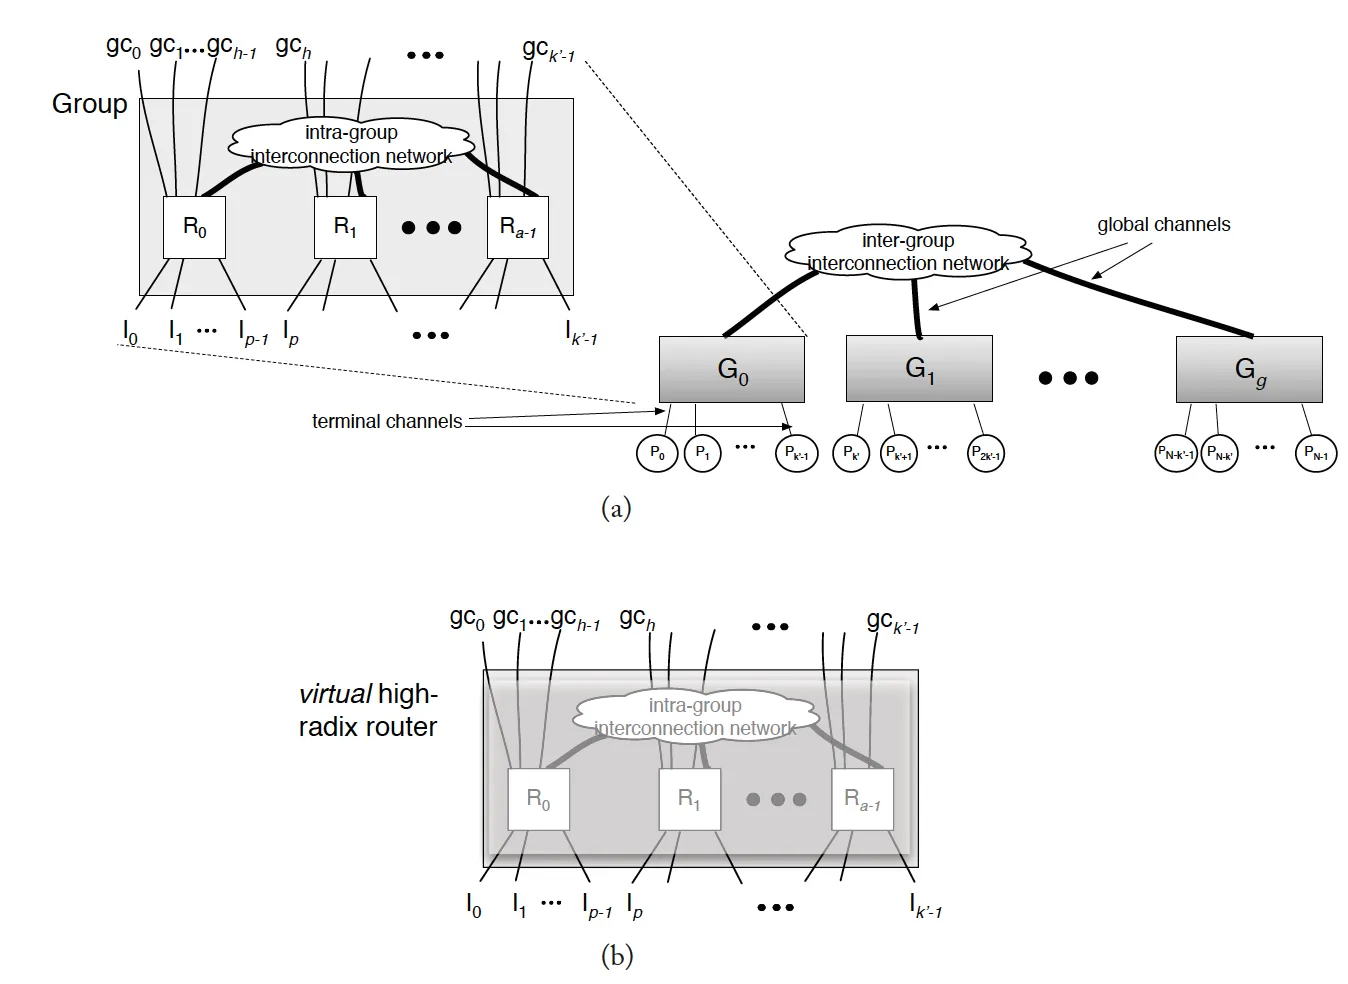
\includegraphics[width=0.8\textwidth]{../assets/ch03/ch03-3_1_网络拓扑-006.png}
\end{figure}
图4.6(b)所示），从而利用输入/输出端口共址的流量局部
性。
然而，Clos或折叠Clos网络的成本几乎是同等容量的蝶形网络的两倍，且延迟更高。成本和延迟的增加
源于数据包需要先路由到任意中间级交换机，再到达最终目的地。这使得网络中的长电缆数量翻倍（成
本约翻倍），并导致穿越的路由器间通道数量翻倍（延迟增加）。
\subsubsection{案例研究：Google Jupiter的演进——从Clos到光交换}

谷歌的数据中心网络架构Jupiter的十年演进，生动展示了Clos拓扑在实际部署中的优势与挑战。2015年，谷歌在SIGCOMM论文中首次披露Jupiter架构，利用商用交换芯片构建五级Clos拓扑，实现了1.3 Pb/s的对分带宽，支持搜索、视频和存储业务的海量需求。

然而，随着规模扩大，Clos拓扑的固有挑战凸显：物理布线复杂性、spine层交换机的高昂成本，以及静态拓扑难以适应动态流量。2022年，谷歌在Jupiter架构中引入了革命性的变革：基于微机电系统（MEMS）的光电路交换机（OCS）。

\textbf{OCS的核心创新}在于将网络拓扑从静态的电域Clos转变为\textbf{动态可重构的直接连接拓扑}。通过OCS，谷歌能够在聚合块之间直接建立光路径，消除了昂贵的spine层电交换机。实际部署表明，这种架构实现了约40\%的功耗降低和30\%的资本支出减少。更重要的是，这种拓扑工程与流量工程的结合，使谷歌能够在不中断业务的情况下实现跨代硬件的平滑升级——这是对传统Clos架构僵化性的根本突破。

谷歌的实践表明，未来的数据中心网络将是"光电混合"的实体：电交换提供细粒度的包级转发，光交换提供大容量的电路级连接。这种融合架构将在AI时代变得愈发重要。

蜻蜓（Dragonfly）拓扑代表了直连网络的最前沿发展，它采用层次化分组设计来优化全局通信。网络被
划分为多个组（Group），组内采用全连接或高维网格，组间则通过稀疏连接形成上层网络。这种结构的
神奇之处在于仅需O(√N)的全局直径，却只需要每个节点3-4个物理端口。美国阿贡国家实验室的"极

                                                            5
光"超算就采用该拓扑，其核心创新在于虚拟通道技术与自适应路由算法的结合，能有效避免热点组间链
路拥塞。




(a) High-level block diagram of dragonfly topology and (b) a virtual high-radix router.
蜻蜓是一种三级分层网络：路由器级、组级和系统级（如上图）。底层每个路由器有三种连接：1)连接到
p个终端；2)通过a−1条本地通道连接到同组其他路由器；3)通过h条全局通道连接到其他组的路由器。因
此，每个路由器的基数（或度数）为k=p+a+h−1。一个组由a个路由器通过本地通道形成的组内互联网络
组成。每组有ap个终端连接和ah个全局通道连接，组内所有路由器共同充当基数为k'=a(p+h)的虚拟路由
器。如上图(b)所示，若忽略组内细节，一个组可视为一个超高基数虚拟路由器（k'>>k）。这种超高基数
使系统级网络能以极低的全局直径（任意两节点间最短路径上昂贵全局通道的最大数量）实现。最多可
连接g=ah+1个组（N=ap(ah+1)个终端），全局直径为1。相比之下，直接用基数k路由器构建的系统级网
络需要更大的全局直径。
在最大规模（N=ap(ah+1)）的蜻蜓网络中，每组间恰好有一条连接。在较小规模的蜻蜓中，每组的全局
连接数超过其他组数量。这些多余的全局连接会均匀分配到各组，确保每组间至少有⌊(ah+1)/g⌋条通
道。蜻蜓参数a、p和h可任意取值，但为在负载均衡流量下平衡通道负载，应满足a=2p=2h。由于每个数
据包在路由中会穿越两条本地通道（全局通道两端各一条）、一条全局通道和一条终端通道，这一比例
能维持平衡。蜻蜓拓扑的路由和负载均衡细节将在第5章讨论。由于全局通道成本高，若偏离2:1的比例，
应超额配置本地和终端通道，以确保昂贵的全局通道充分利用。即网络应满足a≥2h且2p≥2h。通过提高
有效基数，蜻蜓拓扑具有高度可扩展性——使用基数64路由器时，拓扑可扩展至超过256k节点，网络直
径仅为三跳。相比之下，使用基数64路由器的二维扁平化蝶形网络最多扩展至约10k节点，三维版本仅能
扩展至64k节点。

超立方体（hypercube）如图所示，网络中的每个节点可视为一个二进制数。仅有一位数字不同的节点
相互连接。更具体地说，如果两个节点在第 i 位数字上存在差异，则它们在第i维度上相连。在超立方体

                                                                                     6
中，当源节点与目标节点在每个维度上都不同时（例如从图中的000跳转到111），最小路由最多需要
n   跳。然而平均而言，数据包将经历 n/2 跳。




超立方体扩展（HyperX）拓扑扩展了扁平化蝶形，形成更通用的拓扑类别。与扁平化蝶形类似，HyperX
中每维的所有路由器均与同维其他节点全连接，但允许不同维度的交换机数量不同。下图展示了一个
HyperX拓扑示例（L=2维，每维交换机数S1=2、S2=4，集中度T=4，即每个交换机连接4个终端）。定
义HyperX拓扑的另一参数是K，表示每维通道的相对带宽（以终端带宽为单位）。图中假设K=1（所有通
道带宽相等），但若K=2，交换机间通道带宽将是终端通道的2倍。HyperX拓扑可通过四个参数
（L,S,K,T）描述，其中S和K在各维可取值相同（如S1=S2=…=s）形成规则HyperX，或取值不同形成不
规则HyperX。例如，n维超立方体可描述为（L=n,S=2,K=1,T=1），k元n维扁平化蝶形可描述为
（L=n,T=S=k,K=2）。




                                                       7
8


[新增-2026-03] 数据中心网络拓扑

云计算数据中心的网络拓扑与传统企业网络有显著不同。传统数据中心网络主要承载客户机/服务器模式的应用服务，一般采用2层或3层的树形结构（核心层、汇聚层、接入层）。然而，这种传统树形层次结构存在多方面局限性：所有服务器位于同一个2层广播域中；汇聚和核心交换机是服务器之间通信的带宽瓶颈；易于发生"单点故障"。

随着云计算的发展，数据中心网络需要支持：
 ● 超大规模：计算节点数量达到10^5以上量级，交换节点接近10^4量级
 ● 高带宽：服务器之间需要多条通信路径，对分带宽需求巨大
 ● 东西流量主导：数据中心内部流量（东西向）远超进出流量（南北向），比例可达3:1甚至更高
 ● 虚拟机动态迁移：支持VMotion等技术的网络连通性需求

因此，现代数据中心网络拓扑主要采用以下设计：

[新增-2026-03] Fat-Tree拓扑

Fat-Tree是对传统树形层次结构的优化，由Al-Fares等人提出。它仍然分为核心、汇聚和接入3个层次，但具有以下独特之处：

 ● 采用大量统一的廉价商业交换机作为转发设备，避免纵向扩展的高成本
 ● 所有汇聚和接入交换机被划分为不同的集群Pod（k/2台汇聚交换机、k/2台接入交换机），集群内采用全相连方式
 ● 采用多路径路由技术，为服务器之间通信提供较大的对分带宽

Fat-Tree网络中，为实现多路径通信，采用特定的地址分配规则和两级路由表机制。假设使用10.0.0.0/8地址块，Pod内交换机地址形式为10.pod.switch.1，核心交换机地址形式为10.k.j.i，服务器地址形式为10.pod.switch.ID。

[新增-2026-03] Facebook数据中心架构

对于社交网络等特定应用，数据中心的东西流量远超南北流量（可能超出近1000倍）。Fat-Tree结构在这种情况下存在局限性：纵向扩展成本高；昂贵转发设备仍无法有效支撑。

Facebook数据中心采用新型网络结构：
 ● 全面部署廉价架顶交换机（TOR）
 ● 每台架顶交换机以40GBps上行链路与光纤交换机相连
 ● 设计4个相互独立的Spine交换机平面（每个平面可扩展至48台设备）
 ● 集群Pod和骨干平面Spine Plane组成模块化网络拓扑

这种结构通过增加Server Pod实现数据中心扩展，通过增加Spine Plane增加服务器间通信对分带宽。

[新增-2026-03] 无线数据中心网络

随着网络规模扩大，传统有线静态链路面临挑战：布线复杂、难以应对突发流量、改动成本高。无线通信技术为这些问题提供新思路。

60GHz无线通信技术：
 ● 拥有近7GHz宽的可用频谱，可提供Gbps量级速度
 ● 具有抗干扰、防监听特性
 ● 采用有向天线技术、波束成形和波束转向优化链路
 ● 3D-beamforming技术采用反射点到点形式，避免视线链路受障碍物阻塞

自由空间光通信（FSO）：使用可调制的可见或红外光束在自由空间传输，实现更大范围高速传输，避免信号干扰。

[新增-2026-03] 非规则网络结构

REWIRE是针对数据中心网络架构设计的框架，通过优化算法设计无组织、非规则的网络结构：
 ● 在满足用户自定义约束的同时实现最大对分带宽
 ● 最小化端到端延迟
 ● 适用于在现有数据中心基础上进行扩展的场景

REWIRE优化算法分为4步：确定满足约束的网络结构空间；随机选取候选结构；执行local search优化；循环直至找到近似最优结构。

\section{万卡集群的网络拓扑}

随着AI大模型训练规模的指数级增长，单一数据中心的GPU集群已从千卡级别迈向万卡甚至十万卡级别。构建如此规模的训练网络，不仅需要解决单机房的网络架构问题，更需要面对跨机房、跨区域的超大规模互联挑战。本节介绍面向万卡级AI集群的网络拓扑设计。

\subsection{BAG（Backend Aggregation）架构}

BAG（Backend Aggregation，后端聚合）是Meta在其Prometheus等吉瓦级AI集群中采用的核心网络架构技术。它作为集中式的以太网超级汇聚层（Super Spine），负责互联多个Spine层网络，实现跨数据中心和区域的GPU资源池化。

\subsubsection{BAG的定位与功能}

在大型AI集群的分层网络架构中，BAG位于关键的战略位置：

\begin{itemize}
    \item \textbf{区域互联枢纽}：BAG层作为区域网络与主干网络的汇聚点，将分布在多个数据中心的L2网络互联成统一的超级集群
    \item \textbf{容量聚合}：支持Petabit级别的互联带宽（例如，每对区域之间可达16-48 Pbps）
    \item \textbf{统一资源视图}：通过BAG互联，不同物理位置的GPU对上层应用呈现为统一的计算资源池
\end{itemize}

\subsubsection{平面拓扑与分布式拓扑}

BAG层在物理部署上采用分布式架构，以适应大规模集群的需求：

\textbf{平面连接拓扑（Planar Topology）}：BAG交换机在不同区域之间按平面一一对应连接。这种拓扑管理简单，但潜在故障域较为集中。

\textbf{分布式连接拓扑（Spread Connection Topology）}：将链路分散到多个BAG交换机和平面中，提供更丰富的路径多样性和更高的可靠性。当某个BAG交换机或链路故障时，流量可以迅速切换到其他可用路径。

\subsection{跨区域数据中心互联}

BAG架构的核心价值在于支持跨区域的超大规模GPU互联。以Meta的Prometheus集群为例：

\subsubsection{分层互联模型}

\begin{enumerate}
    \item \textbf{建筑内互联}：通过DSF L2网络实现单个建筑内数千GPU的互联
    \item \textbf{区域内互联}：通过BAG层将同一区域的多个建筑互联，形成L3域
    \item \textbf{跨区域互联}：通过BAG-to-BAG连接实现地理分散的数据中心资源的统一调度
\end{enumerate}

\subsubsection{距离与延迟考量}

BAG的分布式架构设计充分考虑了延迟约束：

\begin{itemize}
    \item BAG层与L2边缘之间的距离保持较短，这对于浅缓冲区的NSF（Non-Scheduled Fabric）交换机尤为重要
    \item BAG-to-BAG之间的长距离链路需要采用深缓冲区交换机，以支持PFC等无损拥塞控制协议
    \item 通过优化光纤路由和传输设备，将跨区域延迟控制在RDMA通信可接受的范围内
\end{itemize}

\subsection{多级Clos网络与超配比设计}

万卡级集群的网络拓扑通常采用多级Clos架构的变体，并在不同层级采用差异化的超配比（Oversubscription Ratio）设计。

\subsubsection{三级Clos与超配比}

在典型的万卡集群中，网络通常采用三级架构：

\begin{enumerate}
    \item \textbf{L1层（ToR到Leaf）}：通常采用1:1的无阻塞设计，确保服务器到网络的第一跳带宽充足
    \item \textbf{L2层（Leaf到Spine）}：根据流量模型采用适度的超配比，典型值为4.5:1
    \item \textbf{L3层（Spine到BAG）}：由于跨区域流量相对较小，可以采用更高的超配比（如4.98:1），以降低成本
\end{enumerate}

超配比的选择基于AI训练流量的特征：在数据并行和模型并行训练中，大部分通信发生在同一节点组内，跨区域流量相对有限。因此，适度的高超配比可以在不明显影响性能的情况下显著降低网络成本。

\subsubsection{路由与负载均衡}

BAG架构采用eBGP作为路由协议，并引入链路带宽属性实现UCMP（Unequal Cost Multipath，不等价多路径）：

\begin{itemize}
    \item 根据链路实际带宽进行加权负载分担
    \item 支持动态适应链路故障和带宽变化
    \item BAG-to-BAG连接采用MACsec加密，满足网络安全要求
\end{itemize}

\subsection{混合Fabric架构}

在实际部署中，大型AI集群往往同时采用多种Fabric技术：

\textbf{DSF与NSF的融合}：Meta的Prometheus集群同时部署了DSF（Disaggregated Scheduled Fabric）和NSF（Non-Scheduled Fabric）两种网络：
\begin{itemize}
    \item DSF用于需要高性能、无损传输的训练网络
    \item NSF用于对延迟要求相对宽松的其他后端流量
\end{itemize}

BAG层作为统一的汇聚点，将不同类型的L2网络无缝互联。这种混合架构允许根据具体应用场景选择最合适的网络技术，实现性能与成本的最佳平衡。

\subsection{网络可靠性设计}

万卡级集群的网络可靠性设计需要在多个层面进行考量：

\textbf{故障域分析}：在BAG、数据大厅和电力分配等多个层面进行全面的故障模式分析，确保单点故障不会影响整体训练任务。

\textbf{黑洞避免}：采用多种策略防止路由黑洞，包括：
\begin{itemize}
    \item 受影响的BAG平面流量排空（Draining）
    \item 条件性路由聚合，避免汇聚后的路由震荡
    \item 快速故障检测和路由收敛机制
\end{itemize}

\textbf{增量扩展}：BAG架构支持集群的渐进式扩展。随着AI模型规模的增长，可以通过增加BAG节点和互联链路逐步扩展网络容量，而无需对现有架构进行大规模改造。

\section{[新增-2026-03] AI计算网络创新拓扑}

随着AI大模型训练规模的快速增长，传统数据中心网络拓扑面临成本高、扩展性受限等挑战。华为研究团队在计算网络拓扑领域进行了深入探索，提出了一系列面向AI场景的创新拓扑结构。本节介绍HammingMesh、KNS、Slim Fly和PolarFly四种前沿拓扑，它们在成本、性能和扩展性方面各具特色。

\subsection{HammingMesh拓扑}

HammingMesh是一种专为AI计算集群设计的分层网络拓扑，其核心思想是结合低成本本地互联与高扩展性全局拓扑。该拓扑采用双层架构：本地组（Local Group）使用2D mesh结构，全局层使用Clos拓扑。

\textbf{拓扑参数定义}：HammingMesh由四元组$(a,b,x,y)$定义，其中：
\begin{itemize}
    \item $(a,b)$：本地2D mesh的维度，即每个本地组包含$a \times b$个计算节点
    \item $(x,y)$：全局2D Clos网络的维度
\end{itemize}

\textbf{核心特点}：
\begin{enumerate}
    \item \textbf{低成本本地互联}：本地组内采用PCB铜线直接连接计算芯片，无需昂贵的光模块和交换机，显著降低硬件成本
    \item \textbf{分层解耦设计}：本地通信与全局通信物理分离，本地流量不占用全局网络带宽
    \item \textbf{可扩展全局架构}：利用成熟的Clos拓扑实现全局高对分带宽
\end{enumerate}

\textbf{性能与成本分析}：
\begin{itemize}
    \item All-to-all性能约为同等规模Clos网络的20\%
    \item 相比Dragonfly拓扑成本降低50\%
    \item 相比Clos网络成本降低80\%
\end{itemize}

HammingMesh适用于以本地通信为主、对全局all-to-all性能要求不极致的AI训练场景，如数据并行和流水线并行训练。

\subsection{KNS拓扑}

KNS（K-ary n-dimensional Switched network）拓扑与HammingMesh设计理念相似，但在本地组互联方式上有所区别。KNS在本地组内部使用交换机进行互联，而非直接PCB连接，全局层采用n维Clos拓扑。

\textbf{拓扑特点}：
\begin{itemize}
    \item 本地组通过交换机互联，提供比PCB直连更高的灵活性
    \item 支持n维Clos全局拓扑，扩展性优于2D结构
    \item 2D KNS成本约为Clos网络的40\%
    \item 对分带宽为Clos的一半，all-to-all性能约为50\%
\end{itemize}

KNS在成本和性能之间取得了更好的平衡，适合需要中等全局通信能力的AI训练场景。

\subsection{Slim Fly拓扑}

Slim Fly是一种基于数学图论优化的高效率拓扑，其核心创新在于利用MMS（McKay-Miller-\v{S}ir\'{a}\v{n}）图构建网络结构，达到接近Moore bound的理论极限。

\textbf{理论基础}：
\begin{itemize}
    \item 基于MMS图构建，该图是已知的最大度数为k、直径为2的图类
    \item 达到Moore bound的$\frac{8}{9}$，接近理论最优
    \item 相比同规模Clos网络，可使用更小基数的交换机实现非阻塞特性
\end{itemize}

\textbf{性能优势}：
\begin{enumerate}
    \item 网络直径仅为2跳，延迟极低
    \item 交换机基数需求小，降低硬件成本和功耗
    \item 路径多样性丰富，支持自适应路由
\end{enumerate}

Slim Fly拓扑特别适合对延迟极度敏感的AI推理场景和小规模高速互联场景。

\subsection{PolarFly拓扑}

PolarFly是另一种基于数学图论的前沿拓扑，采用ER（Erd\H{o}s-R\'{e}nyi）极性图作为构建基础。

\textbf{核心特性}：
\begin{itemize}
    \item 基于ER极性图构建，具有优良的对称性和扩展性
    \item 渐进接近Moore bound，在大规模部署时性能优势更加明显
    \item 支持灵活的端口配置，适配不同规模集群需求
\end{itemize}

\subsection{创新拓扑对比分析}

表~\ref{tab:topology_comparison}对上述创新拓扑进行了综合对比：

\begin{table}[htbp]
\centering
\caption{AI计算网络创新拓扑对比}
\label{tab:topology_comparison}
\begin{tabular}{|l|c|c|c|c|c|}
\hline
\textbf{拓扑类型} & \textbf{成本(相对Clos)} & \textbf{对分带宽} & \textbf{All-to-all性能} & \textbf{网络直径} & \textbf{适用场景} \\
\hline
Clos（基准） & 100\% & 100\% & 100\% & $2\log_k N$ & 通用高性能计算 \\
\hline
HammingMesh & 20\% & 中等 & 20\% & 本地1跳+全局多跳 & 数据并行训练 \\
\hline
KNS（2D） & 40\% & 50\% & 50\% & 本地2跳+全局多跳 & 混合并行训练 \\
\hline
Slim Fly & 60\% & 80\% & 85\% & 2 & 低延迟推理 \\
\hline
PolarFly & 55\% & 85\% & 90\% & 2-3 & 大规模训练 \\
\hline
Dragonfly & 40\% & 70\% & 75\% & 3 & 超算中心 \\
\hline
\end{tabular}
\end{table}

从表中可以看出，不同拓扑在成本-性能权衡方面各有侧重。HammingMesh以最低成本满足基本互联需求，Slim Fly和PolarFly则在保持较高性能的同时显著降低成本，为AI基础设施建设提供了更多选择。

\section{[新增-2026-03] 软件定义光电网络}

随着AI模型规模指数级增长，传统电交换网络面临功耗、带宽和灵活性等多重挑战。软件定义光电网络（HyperTPE）通过光交叉连接（OXC）技术和智能控制算法，为超大规模AI集群提供了高效、灵活的网络解决方案。

\subsection{OXC光交叉连接技术}

OXC（Optical Cross Connect，光交叉连接）是软件定义光电网络的核心设备，能够在光层实现灵活的信号路由和调度。

\textbf{OXC技术特点}：
\begin{itemize}
    \item \textbf{全光交换}：光信号直接在光域完成交换，无需光电转换，大幅降低功耗和延迟
    \item \textbf{大容量调度}：单台OXC设备可支持数百端口的全互联，满足超大规模集群需求
    \item \textbf{快速重配置}：通过软件控制实现毫秒级光路切换，支持动态拓扑调整
    \item \textbf{波长级粒度}：支持波长选择性交换，实现精细化的带宽分配
\end{itemize}

\subsection{HyperTPE架构}

HyperTPE（Hybrid Programmable Terabit-scale Photonic-Electronic network）是华为提出的软件定义光电融合网络架构。

\textbf{架构层次}：
\begin{enumerate}
    \item \textbf{光电融合交换层}：OXC负责长距离、大带宽的光路连接，电交换机处理短距离、细粒度流量
    \item \textbf{智能控制层}：集中式控制器统一管理光路和电路资源
    \item \textbf{应用接口层}：提供北向API，支持AI训练框架对网络资源的按需调用
\end{enumerate}

\subsection{拓扑动态重构算法}

HyperTPE的核心能力在于根据AI训练流量特征动态重构网络拓扑。

\textbf{BvN矩阵分解算法}：
基于Birkhoff-von Neumann定理，将流量矩阵分解为多个置换矩阵的凸组合：
\begin{equation}
    T = \sum_{i=1}^{k} \alpha_i P_i, \quad \sum_{i=1}^{k} \alpha_i = 1
\end{equation}
其中$T$为流量矩阵，$P_i$为置换矩阵，$\alpha_i$为权重系数。该分解结果可直接映射为光拓扑配置。

\textbf{贪心流量分配算法}：
对于粗粒度流量分配，采用贪心算法进行优化：
\begin{enumerate}
    \item 按流量大小对通信对排序
    \item 优先为流量大的通信对分配专用光路
    \item 剩余流量通过电交换网络承载
\end{enumerate}

\textbf{拓扑重配置优化模型}：
建立混合整数线性规划（MILP）模型求解最优拓扑：
\begin{align}
    \min_{x,y} \quad & \sum_{i,j} c_{ij}x_{ij} + \lambda \sum_{i,j,k} d_{ijk}y_{ijk} \\
    \text{s.t.} \quad & \sum_{k} y_{ijk} \geq t_{ij}, \quad \forall i,j \\
    & x_{ij} \in \{0,1\}, \quad y_{ijk} \geq 0
\end{align}
其中$x_{ij}$表示光路配置决策，$y_{ijk}$表示流量分配，$t_{ij}$为流量需求。

\textbf{性能指标}：
\begin{itemize}
    \item 256 Pod规模网络：分钟级拓扑计算
    \item 重配置时间减少30\%
    \item 整体网络利用率提升25\%
\end{itemize}

软件定义光电网络为AI大模型训练提供了灵活高效的网络基础设施，代表了数据中心网络演进的重要方向。
